\documentclass[10pt, a4paper]{article} % Set base size to 10pt

\usepackage[utf8]{inputenc} 
\usepackage[T1]{fontenc}    

% --- Arial/Helvetica Setup ---
\usepackage{helvet}               % Load Helvetica (Arial clone)
\renewcommand{\familydefault}{\sfdefault} % Set default font to Sans-Serif
% -----------------------------

\usepackage{graphicx}  
\usepackage{booktabs}    
\usepackage{amsmath}               
\usepackage{hyperref}      
\usepackage{multirow}
\usepackage{multicol}
\usepackage{subcaption}
\usepackage{amssymb}
\usepackage[a4paper, margin=1in]{geometry}
\usepackage{parskip}

% \usepackage{cite} 
\usepackage[
    style=authoryear, % Or 'numeric', 'apa', etc.
    maxbibnames=5,    % Show max 5 authors in the bibliography
    minbibnames=1,    % If more than 5, shorten to just 1 author + et al.
    maxcitenames=2,   % Show max 2 authors in the text citation
    mincitenames=1,   % If more than 2, shorten to 1 author + et al.
    backend=biber
]{biblatex}
\addbibresource{references.bib}


\title{CelebAMask Face Parsing}

\author{
    ARDACANDRA SUBIANTORO (G2505312G)
    \and   
    College of Computing and Data Science \\
    Nanyang Technological University, Singapore \\
    \texttt{ARDA0001@e.ntu.edu.sg}
}
\date{} 



\begin{document}

\maketitle

\section{Introduction}
Face parsing is a pixel-wise semantic segmentation task aimed at assigning discrete labels to facial components, such as the skin, nose, and eyes. This project utilizes the CelebAMask-HQ dataset \parencite{CelebAMask-HQ}, employing a restricted subset of 1,000 training and 100 validation image-mask pairs at a 512x512 resolution, with final performance evaluated on 100 test pairs using the F-measure. Since the validation set ground-truth is not given, the training pairs are further split with a 90:10 ratio for development iteration evaluations.

To emphasize architectural efficiency and fundamental model design, the project applies a strict limit of 1,821,085 trainable parameters. Furthermore, the development prohibits the use of external data, pretrained weights, or ensemble modeling techniques.

\section{Baseline Model: SRResNet}
The baseline architecture for this project is based on the SRResNet \parencite{ledig2017photorealisticsingleimagesuperresolution}, adapted from its original super-resolution context to the task of semantic segmentation. The model is structured into four primary stages: 

\begin{enumerate}
    \item \textbf{Initial Feature Extraction:} A convolutional layer utilizing a large 9x9 kernel to capture a wide initial spatial context.
    \item \textbf{Residual Backbone:} A series of 16 Residual Blocks designed to facilitate robust gradient flow and high-level feature learning.
    \item \textbf{Context Module:} A sequence of dilated convolutions with dilation rates of 2, 4, and 8. These allow the model to significantly expand its receptive field without losing the high-resolution spatial information required for pixel-wise accuracy.
    \item \textbf{Decoder and Head:} A multi-stage decoder that progressively reduces channel depth ($64 \to 48 \to 32$) before a final 1x1 convolutional segmentation head produces the raw logits for the 19 semantic classes.
\end{enumerate}

A key advantage of this specific configuration is that it entirely avoids downsampling (strided convolutions or pooling). By maintaining the full 512x512 resolution throughout the network, the model preserves details better, leading to more precise boundary separation in the resulting face parsing masks.

\section{Data Augmentation Experimentation}

To mitigate the risk of overfitting and improve model regularization given the small training set of 1,000 images, several data augmentation strategies were evaluated. Both spatial and pixel-level transformations were investigated to assess their impact on model generalization:

\begin{itemize}
    \item \textbf{Spatial Transformations:} Horizontal flipping, random rotation, and spatial shifting.
    \item \textbf{Pixel-level Transformations:} Adjustments to contrast and brightness.
\end{itemize}

The results of these experiments, measured by the F-score on the validation set, are summarized in Table~\ref{tab:augmentation}.

\begin{table}[h]
\centering
\caption{Comparison of F-score across different augmentation iterations (10 epochs, batch size 4, 256x256 input image).}
\label{tab:augmentation}
\begin{tabular}{@{}lc@{}}
\toprule
Augmentation Strategy & F-score \\ \midrule
Baseline (No Augmentation) & 0.4599 \\
Horizontal Flip & 0.4581 \\
\textbf{Rotation} & \textbf{0.5762} \\
\textbf{Shifting} & \textbf{0.5853} \\
\textbf{Contrast} & \textbf{0.5847} \\ 
Brightness Adjustments & 0.5387 \\ \bottomrule
\end{tabular}
\end{table}

The experimental data reveals that **Horizontal Flip** slightly degrades performance, likely due to the semantic distinction between asymmetrical classes (e.g., left vs. right eye) which becomes inverted during flipping. 

In contrast, **Shifting** and **Rotation** provided the most substantial performance gains, increasing the F-score by approximately 27\%. This indicates that even in well-aligned datasets like CelebAMask-HQ, introducing spatial variance forces the model to learn more robust, translation-invariant facial features. **Contrast** adjustments also yielded high performance, suggesting that enhancing edge-gradient visibility helps the model parse in more detail. Shifting, Rotation, and Contrast were selected for the final training pipeline.

\section{Loss Function Analysis}

Face parsing often suffers from significant class imbalance, where large regions such as "skin" dominate the pixel count compared to smaller, critical features like "eyes." To address this, several loss functions and their combinations are evaluated:

\begin{enumerate}
    \item \textbf{Cross-Entropy (CE):} The baseline pixel-wise classification loss, defined as:
    \begin{equation}
        L_{CE} = -\sum_{c=1}^C y_{i,c} \log(\hat{y}_{i,c})
    \end{equation}
    where $y$ is the ground truth and $\hat{y}$ is the predicted probability for class $c$.

    \item \textbf{Dice Loss:} Designed to maximize the overlap between predicted masks ($p$) and ground-truth ($g$), using a smoothing factor of $1.0$:
    \begin{equation}
        L_{Dice} = 1 - \frac{2 \sum p_i g_i + \epsilon}{\sum p_i^2 + \sum g_i^2 + \epsilon}
    \end{equation}

    \item \textbf{Focal Loss:} Focused on "hard" pixels at boundaries by down-weighting easy samples, utilizing $\alpha=0.75$ and $\gamma=2.5$:
    \begin{equation}
        L_{Focal} = -\alpha(1 - \hat{y}_t)^\gamma \log(\hat{y}_t)
    \end{equation}

    \item \textbf{Boundary-Aware Loss:} Specifically targeting edge precision using a Laplacian kernel to extract boundaries, using a dilation of 5, with $w_{CE}=1.0$ and $w_{boundary}=2.0$.

    \item \textbf{Hybrid (CE + Dice + Boundary):} A weighted combination designed to leverage global stability and local refinement.
\end{enumerate}

The performance of each configuration is summarized in Table~\ref{tab:loss_results}.

\begin{table}[h]
\centering
\caption{F-score performance comparison across various loss functions (10 epochs, batch size 4, 256x256 input image).}
\label{tab:loss_results}
\begin{tabular}{@{}lc@{}}
\toprule
Loss Function Configuration & F-score \\ \midrule
Baseline (Cross-Entropy) & 0.5536 \\
Dice Loss & 0.1916 \\
Focal Loss & 0.5504 \\
Boundary-Aware Loss & 0.4744 \\
\textbf{Hybrid (CE + Dice + Boundary)} & \textbf{0.6253} \\ \bottomrule
\end{tabular}
\end{table}

The experiments revealed that using Dice, Focal, or Boundary-Aware loss in isolation actually reduced model performance. This suggests that without the stable gradient of Cross-Entropy, these specialized losses can lead to training instability on a small dataset. However, the **Hybrid** approach yielded the best results. By combining the strengths of each—$L_{CE}$ for global category consistency, $L_{Dice}$ for class imbalance, and $L_{Boundary}$ for edge refinement—the model achieved superior boundary delineation while maintaining high overall classification accuracy. For this reason, the CE + Dice + Boundary loss was selected for the final training pipeline.

\section{Model Architecture Modification: Lite-Face Parser}

The \textbf{Lite-Face Parser (LFP)} is a lightweight, multi-path segmentation architecture optimized for face parsing under strict parameter constraints. It employs a \textbf{Context Path} featuring Inverted Residuals and a \textbf{LiteASPP} module to capture global dependencies, while parallel \textbf{Detail} and \textbf{Texture Paths} preserve fine-grained spatial features. These representations are integrated via a \textbf{Bidirectional Decoder} with \textbf{Weighted Bi-Fusion} and a class-aware \textbf{Prototype Refinement} module, ensuring high-fidelity segmentation across both majority and minority facial classes.

\begin{figure*}[h]
    \centering
    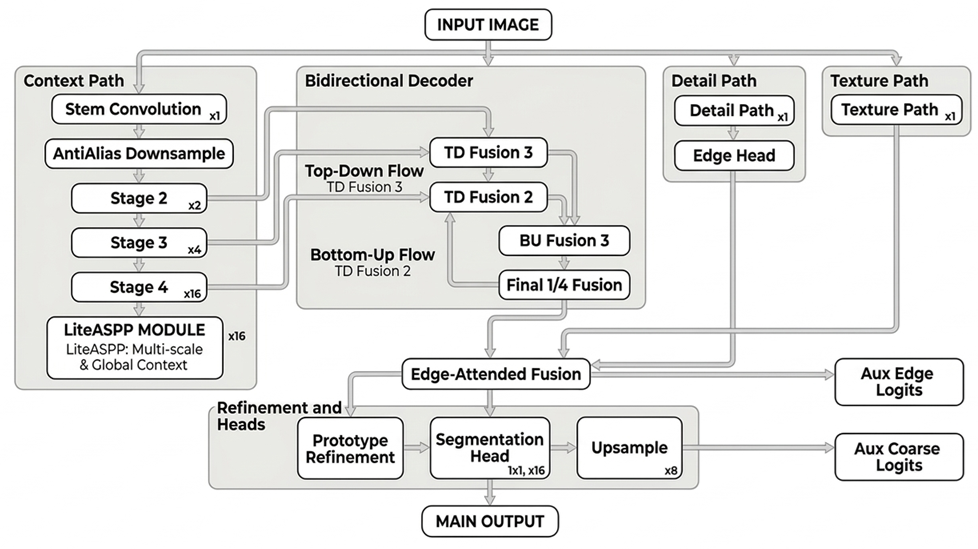
\includegraphics[width=\textwidth]{img/lite_face_parser_v2_diagram_gemini.png}
    \caption{Architecture diagram of the Lite-Face Parser, showcasing the multi-path segmentation consisting of Context Path, Detail Path, and Texture Path.}
    \label{fig:lfp_diagram}
\end{figure*}

\subsection{Architectural Core Concepts}
The LFP architecture leverages several key innovations in efficient deep learning:
\begin{itemize}
    \item \textbf{Inverted Residual Bottlenecks:} Following the principles of MobileNetV2 \parencite{sandler2019mobilenetv2invertedresidualslinear}, the Context Path uses bottleneck blocks that perform a 1x1 expansion, 3x3 depthwise convolution, and 1x1 linear projection. This ensures information flows through narrow manifolds without significant loss.
    \item \textbf{LiteASPP Context:} Inspired by DeepLabV3 \parencite{chen2017rethinkingatrousconvolutionsemantic}, the LiteASPP module provides multi-scale context by concatenating parallel dilated depthwise-separable branches and global image pooling. This allows the model to capture facial features of varying sizes at the deepest feature level.
    \item \textbf{Weighted Bi-Fusion Decoder:} A bidirectional feature pyramid that replaces static concatenation with learnable fusion weights \parencite{tan2020efficientdetscalableefficientobject}. This dynamically balances semantic and spatial cues to optimize feature integration across varying scales.
    \item \textbf{Detail and Texture Paths:} Parallel shallow branches at 1/4 resolution that preserve high-frequency spatial information. These paths isolate boundary-sensitive edges and subtle surface patterns to counteract the spatial loss inherent in the deep context encoder.
    \item \textbf{Prototype Refinement:} A class-aware attention module that computes global feature centroids (prototypes) to refine pixel-level representations \parencite{wang2020panetfewshotimagesemantic}. This enhances segmentation consistency, particularly for minority facial classes and ambiguous boundaries.
    \item \textbf{Edge-Guided Fusion:} A gating mechanism that utilizes an auxiliary edge attention map to sharpen transitions. It modulates the final fusion of context, detail, and texture features to ensure high-fidelity boundaries between adjacent facial components.
\end{itemize}

\subsection{Quantitative and Qualitative Evaluation}
The LFP model was evaluated against the SRResNet baseline using a 512x512 input resolution and 19 semantic classes. As demonstrated in Table \ref{tab:model_comparison}, the LFP architecture achieves a significantly higher F-score of 0.7429 compared to 0.6357 for the baseline.

\begin{table}[h]
\centering
\caption{F-score performance comparison between baseline and new architecture (30 epochs, 512x512 input image, hybrid loss, with data augmentation).}
\label{tab:model_comparison}
\begin{tabular}{@{}lcc@{}}
\toprule
Model Architecture & \# Parameters & F-score \\ \midrule
SRResNet           & 1,428,762     & 0.6357  \\
\textbf{Lite-Face Parser} & \textbf{1,820,207} & \textbf{0.7429} \\ \bottomrule
\end{tabular}
\end{table}

The qualitative comparison in Figure \ref{fig:qualitative_results} highlights the practical benefits of the LFP architecture. While the SRResNet baseline output suffers from significant "blotching" and fragmented class predictions, the LFP model produces much cleaner masks with sharp, well-defined boundaries. This improvement is attributed to the hierarchical fusion of features which preserves structural integrity better than standard residual backbones.

\begin{figure*}[h]
    \centering
    \begin{subfigure}[b]{0.30\textwidth}
        \centering
        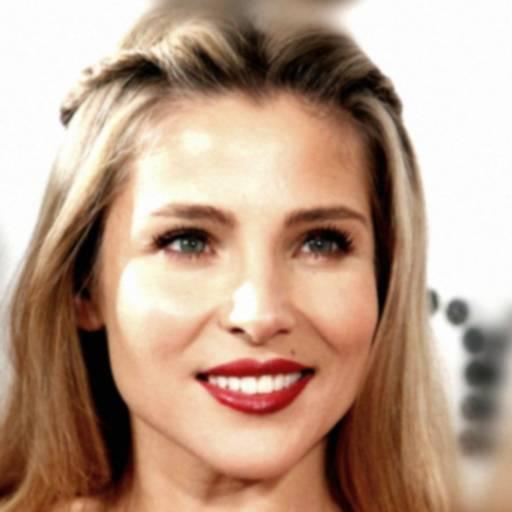
\includegraphics[width=\textwidth]{img/original_image.jpg}
        \caption{Input Image}
    \end{subfigure}
    \hfill
    \begin{subfigure}[b]{0.30\textwidth}
        \centering
        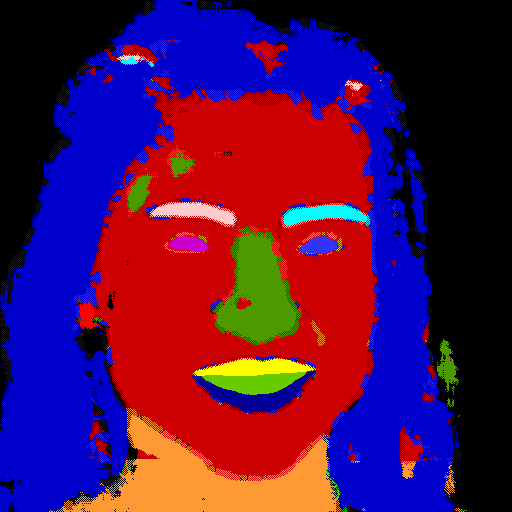
\includegraphics[width=\textwidth]{img/mask_srr.png}
        \caption{SRResNet}
    \end{subfigure}
    \hfill
    \begin{subfigure}[b]{0.30\textwidth}
        \centering
        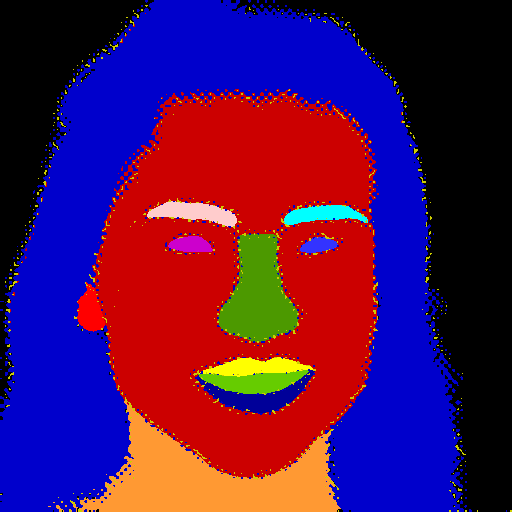
\includegraphics[width=\textwidth]{img/mask_lfp_v2.png}
        \caption{Lite-Face Parser}
    \end{subfigure}
    \caption{Qualitative comparison showing the reduction in segmentation artifacts (blotches) when moving from SRResNet to the Lite-Face Parser.}
    \label{fig:qualitative_results}
\end{figure*}

\subsection{Post-processing}

\begin{figure*}[h]
    \centering
    \begin{subfigure}[b]{0.30\textwidth}
        \centering
        
\includegraphics[width=\textwidth]{img/pp_comp_ori.jpg}
        \caption{Input Image}
    \end{subfigure}
    \hfill
    \begin{subfigure}[b]{0.30\textwidth}
        \centering
        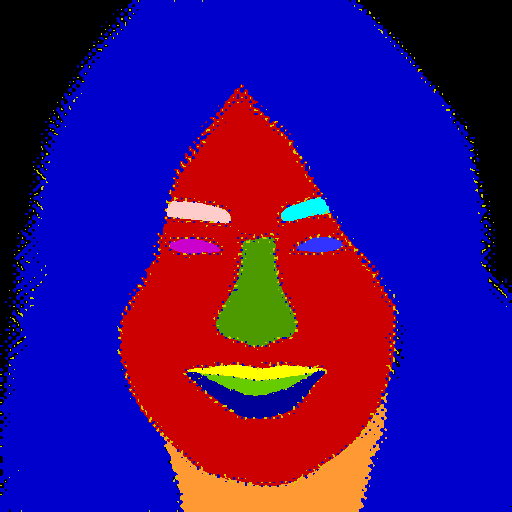
\includegraphics[width=\textwidth]{img/pp_comp_ori_mask.png}
        \caption{Before Post-processing}
    \end{subfigure}
    \hfill
    \begin{subfigure}[b]{0.30\textwidth}
        \centering
        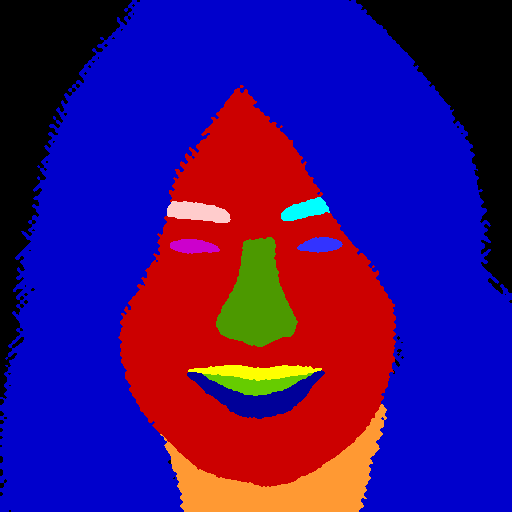
\includegraphics[width=\textwidth]{img/pp_comp_pp_mask.png}
        \caption{After Post-processing}
    \end{subfigure}
    \caption{Qualitative comparison showing the reduction in grains when implementing post-processing.}
    \label{fig:qualitative_results_postprocessing}
\end{figure*}

To refine the segmentation results, a post-processing pipeline was implemented to address the presence of high-frequency noise. The pipeline consists of a combination of small component removal and a 3x3 majority filter to mitigate the artifacts. This approach effectively eliminates insignificant clusters and smooths the boundaries of the segmented regions, resulting in a visually cleaner and more coherent final mask as shown in Figure \ref{fig:qualitative_results_postprocessing}c.

\section{Test Results}
\begin{figure*}[h]
    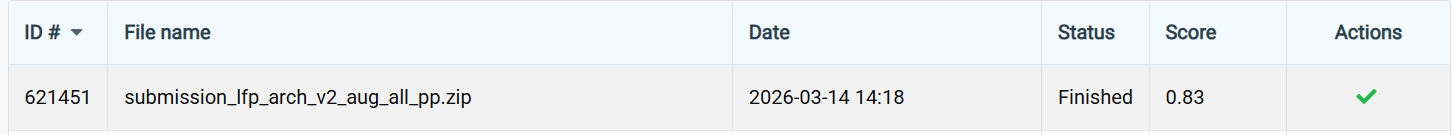
\includegraphics[width=\textwidth]{img/leaderboard_screenshot.png}
    \caption{The Lite-Face Parser model with 1,820,207 parameters is able to achieve a F1-score of 0.83 on the test set.}
    \label{fig:leaderboard_screenshot}
\end{figure*}

\section{Conclusion}
This project successfully developed and evaluated the Lite-Face Parser, a parameter-efficient architecture tailored for high-fidelity face parsing under a strict 1.82M parameter constraint. Through systematic experimentation, it was determined that spatial augmentations (rotation and shifting) and a hybrid loss function (CE + Dice + Boundary) provided the necessary regularization and gradient stability to handle the limited training size of 1,000 images. This work demonstrates that by prioritizing architectural efficiency and boundary-aware loss functions, high-precision semantic segmentation can be achieved even without the use of pretrained weights or massive datasets.

\section{Generative AI Declaration}

The author utilized Gemini 3.0 Pro \parencite{gemini2026} to provide grammatical refinements and perform technical spell-checking across the report. The core experimental design, model development, and the interpretation of the results remain the original work of the author.

% --- References ---
\newpage
\printbibliography

\end{document}